% bei Standalone in documentclass noch:
% \RequirePackage{luatex85}

\documentclass[captions=tableheading, titlepage= firstiscover, parskip = half , bibliography=totoc]{scrartcl}
%paper = a5 für andere optinen
% titlepage= firstiscover
% bibliography=totoc für bibdateien
% parskip=half  Veränderung um Absätze zu verbessern

\usepackage{scrhack} % nach \documentclass
\usepackage[aux]{rerunfilecheck}
\usepackage{polyglossia}
\usepackage[style=numeric, backend=biber]{biblatex} % mit [style = alphabetic oder numeric] nach polyglossia
\addbibresource{lit.bib}
\setmainlanguage{german}

\usepackage[autostyle]{csquotes}
\usepackage{amsmath} % unverzichtbare Mathe-Befehle
\usepackage{amssymb} % viele Mathe-Symbole
\usepackage{mathtools} % Erweiterungen für amsmath
\usepackage{fontspec} % nach amssymb
% muss ins document: \usefonttheme{professionalfonts} % für Beamer Präsentationen
\usepackage{longtable}

\usepackage[
math-style=ISO,    % \
bold-style=ISO,    % |
sans-style=italic, % | ISO-Standard folgen
nabla=upright,     % |
partial=upright,   % /
]{unicode-math} % "Does exactly what it says on the tin."
\setmathfont{Latin Modern Math}
% \setmathfont{Tex Gyre Pagella Math} % alternativ

\usepackage[
% die folgenden 3 nur einschalten bei documenten
locale=DE,
separate-uncertainty=true, % Immer Fehler mit ±
per-mode=symbol-or-fraction, % m/s im Text, sonst \frac
]{siunitx}

% alternativ:
% per-mode=reciprocal, % m s^{-1}
% output-decimal-marker=., % . statt , für Dezimalzahlen

\usepackage[
version=4,
math-greek=default,
text-greek=default,
]{mhchem}

\usepackage[section, below]{placeins}
\usepackage{caption} % Captions schöner machen
\usepackage{graphicx}
\usepackage{grffile}
\usepackage{subcaption}

% \usepackage{showframe} Wenn man die Ramen sehen will

\usepackage{float}
\floatplacement{figure}{htbp}
\floatplacement{table}{htbp}

\usepackage{mhchem} %chemische Symbole Beispiel: \ce{^{227}_{90}Th+}


\usepackage{booktabs}

 \usepackage{microtype}
 \usepackage{xfrac}

 \usepackage{expl3}
 \usepackage{xparse}

 % \ExplSyntaxOn
 % \NewDocumentComman \I {}  %Befehl\I definieren, keine Argumente
 % {
 %    \symup{i}              %Ergebnis von \I
 % }
 % \ExplSyntaxOff

 \usepackage{pdflscape}
 \usepackage{mleftright}

 % Mit dem mathtools-Befehl \DeclarePairedDelimiter können Befehle erzeugen werden,
 % die Symbole um Ausdrücke setzen.
 % \DeclarePairedDelimiter{\abs}{\lvert}{\rvert}
 % \DeclarePairedDelimiter{\norm}{\lVert}{\rVert}
 % in Mathe:
 %\abs{x} \abs*{\frac{1}{x}}
 %\norm{\symbf{y}}

 % Für Physik IV und Quantenmechanik
 \DeclarePairedDelimiter{\bra}{\langle}{\rvert}
 \DeclarePairedDelimiter{\ket}{\lvert}{\rangle}
 % <name> <#arguments> <left> <right> <body>
 \DeclarePairedDelimiterX{\braket}[2]{\langle}{\rangle}{
 #1 \delimsize| #2
 }

\setlength{\delimitershortfall}{-1sp}

 \usepackage{tikz}
 \usepackage{tikz-feynman}

 \usepackage{csvsimple}
 % Tabellen mit \csvautobooktabular{"file"}
 % muss in table umgebung gesetzt werden


% \multicolumn{#Spalten}{Ausrichtung}{Inhalt}

\usepackage{hyperref}
\usepackage{bookmark}
\usepackage[shortcuts]{extdash} %nach hyperref, bookmark

\newcommand{\ua}[1]{_\symup{#1}}
\newcommand{\su}[1]{\symup{#1}}


\title{Versuch 356}
\subtitle{Kettenschaltung mit LC-Gliedern}
\author{Sebastian Pape\\
        sepa@gmx.de \and
        Jonah Nitschke\\
        lejonah@web.de}
\date{Durchführung: 17.01.2017\\
      Abgabe: 24.01.2017}

\begin{document}
\maketitle

\section{Theorie}

In dem folgendem Versuch geht es um die Betrachtung von Wellen mithilfe eine
$LC$-Kette als Analogon zum verketteten harmonischen Oszillators in der
Mechanik. Eine LC-Kette ist eine Kettenschaltung aus mehreren einzelnen LC-Kreise.
Es gibt dabei verschiedenen Betrachtungen solch einer Kette. Einerseits handelt es
sich bei den einzelnen Kettengliedern um Tiefpässe, somit kann ein solche Schaltung
zum Beispiel zum Herausfiltern von hohen Frequenzen genutzt werden.

Andererseits handelt es sich auch um ein gekoppeltes Schwingungssystem, daher eine
Kopplung von Schwingkreisen durch gemeinsame Kapazitäten. Somit kann eine
LC-Kettenschaltung als Transportvorrichtung für elektrische Energie betrachtet werden.
Betrachtet werden soll also, unter welchen Bedingungen Energie nun von einem
zum anderen Ende transportiert werden kann. In dem Versuch wird dabei die als
Dispersion bezeichnete Erscheinung, dass der Energietransport von der angelegten
Frequenz abhängig und nur in endlichen Frequenzbereichen möglich ist, untersucht.

Eine weiter Analogie besteht zu einem mechanischen Schwingungssystem. Somit eignet
sich eine LC-Kette auch zu Darstellung bzw. Betrachtung von Wellen. Dabei werden
verschiedene charakteristische Größen der entstehenden stehenden Wellen betrachtet,
wie zum Beispiel Dispersionsrelation, sowie Phasenverschub zwischen der eingehenden
und ausgehenden Spannung.

\subsection{Die Dispersionsrelationen}

Im Allgemeinen gibt die Dispersionsrelation an, in wie weit verschiedene physikalische
Größen Abhängigkeiten von der Frequenz aufweisen. Um diese Abhängigkeiten für
eine LC-Kettenschaltung zu bestimmen, wird zunächst mithilfe der Kirchoffschen
Regeln die Schwingungsgleichung hergeleitet und auf $n$ Kettenglieder verallgemeinert.
Mit der Annahme, dass alle Kettenglieder mit der gleichen Frequenz $\omega$ schwingen
und lediglich beim Durchlaufen einen Phasenverschub $\theta$ erfahren, lässt sich
für die Kette folgende Dispersionsrelation herleiten:

\begin{equation}
  \omega^2 = \frac{2}{LC}(1-\cos{\theta}) .
  \label{eqn:RelationC}
\end{equation}

Aus dieser Formel lässt sich also die Phasenänderung pro Kettenglied in Abhängigkeit
der angelegten Frequenz bestimmen.

Die bei Formel \eqref{eqn:RelationC} bestimmte Dispersionsrelation lässt
sich etwas verallgemeinern, indem eine Kettenschaltung  mit alternierend eingebauten
Kondensatoren $C\ua{1}$ und $C\ua{2}$ verwendet wird. Bei der Lösung der analog
zu der obigen Schaltung bestimmten Schwingungsgleichung wird hierbei die Annahme
getroffen, dass alle Kettenglieder immernoch mit der gleichen Frequenz schwingen,
allerdings jedes zweite Kettenglied eine andere Amplitude aufweist. Somit ergibt
sich für die $LC\ua{1}C\ua{2}$-Kette folgende Dispersionsrelation:

\begin{equation}
  \omega\ua{1,2}^2 = \frac{1}{L} \left\{ \frac{1}{C\ua{1}} + \frac{1}{C\ua{2}}
  \right\} \, \pm \, \frac{1}{L} \sqrt{ \left\{ \frac{1}{C\ua{1}} + \frac{1}{C\ua{2}}
  \right\}^2  - \frac{4\sin(\theta)^2}{C\ua{1}C\ua{2}}} .
  \label{eqn:RelationC1C2}
\end{equation}

\begin{figure}
  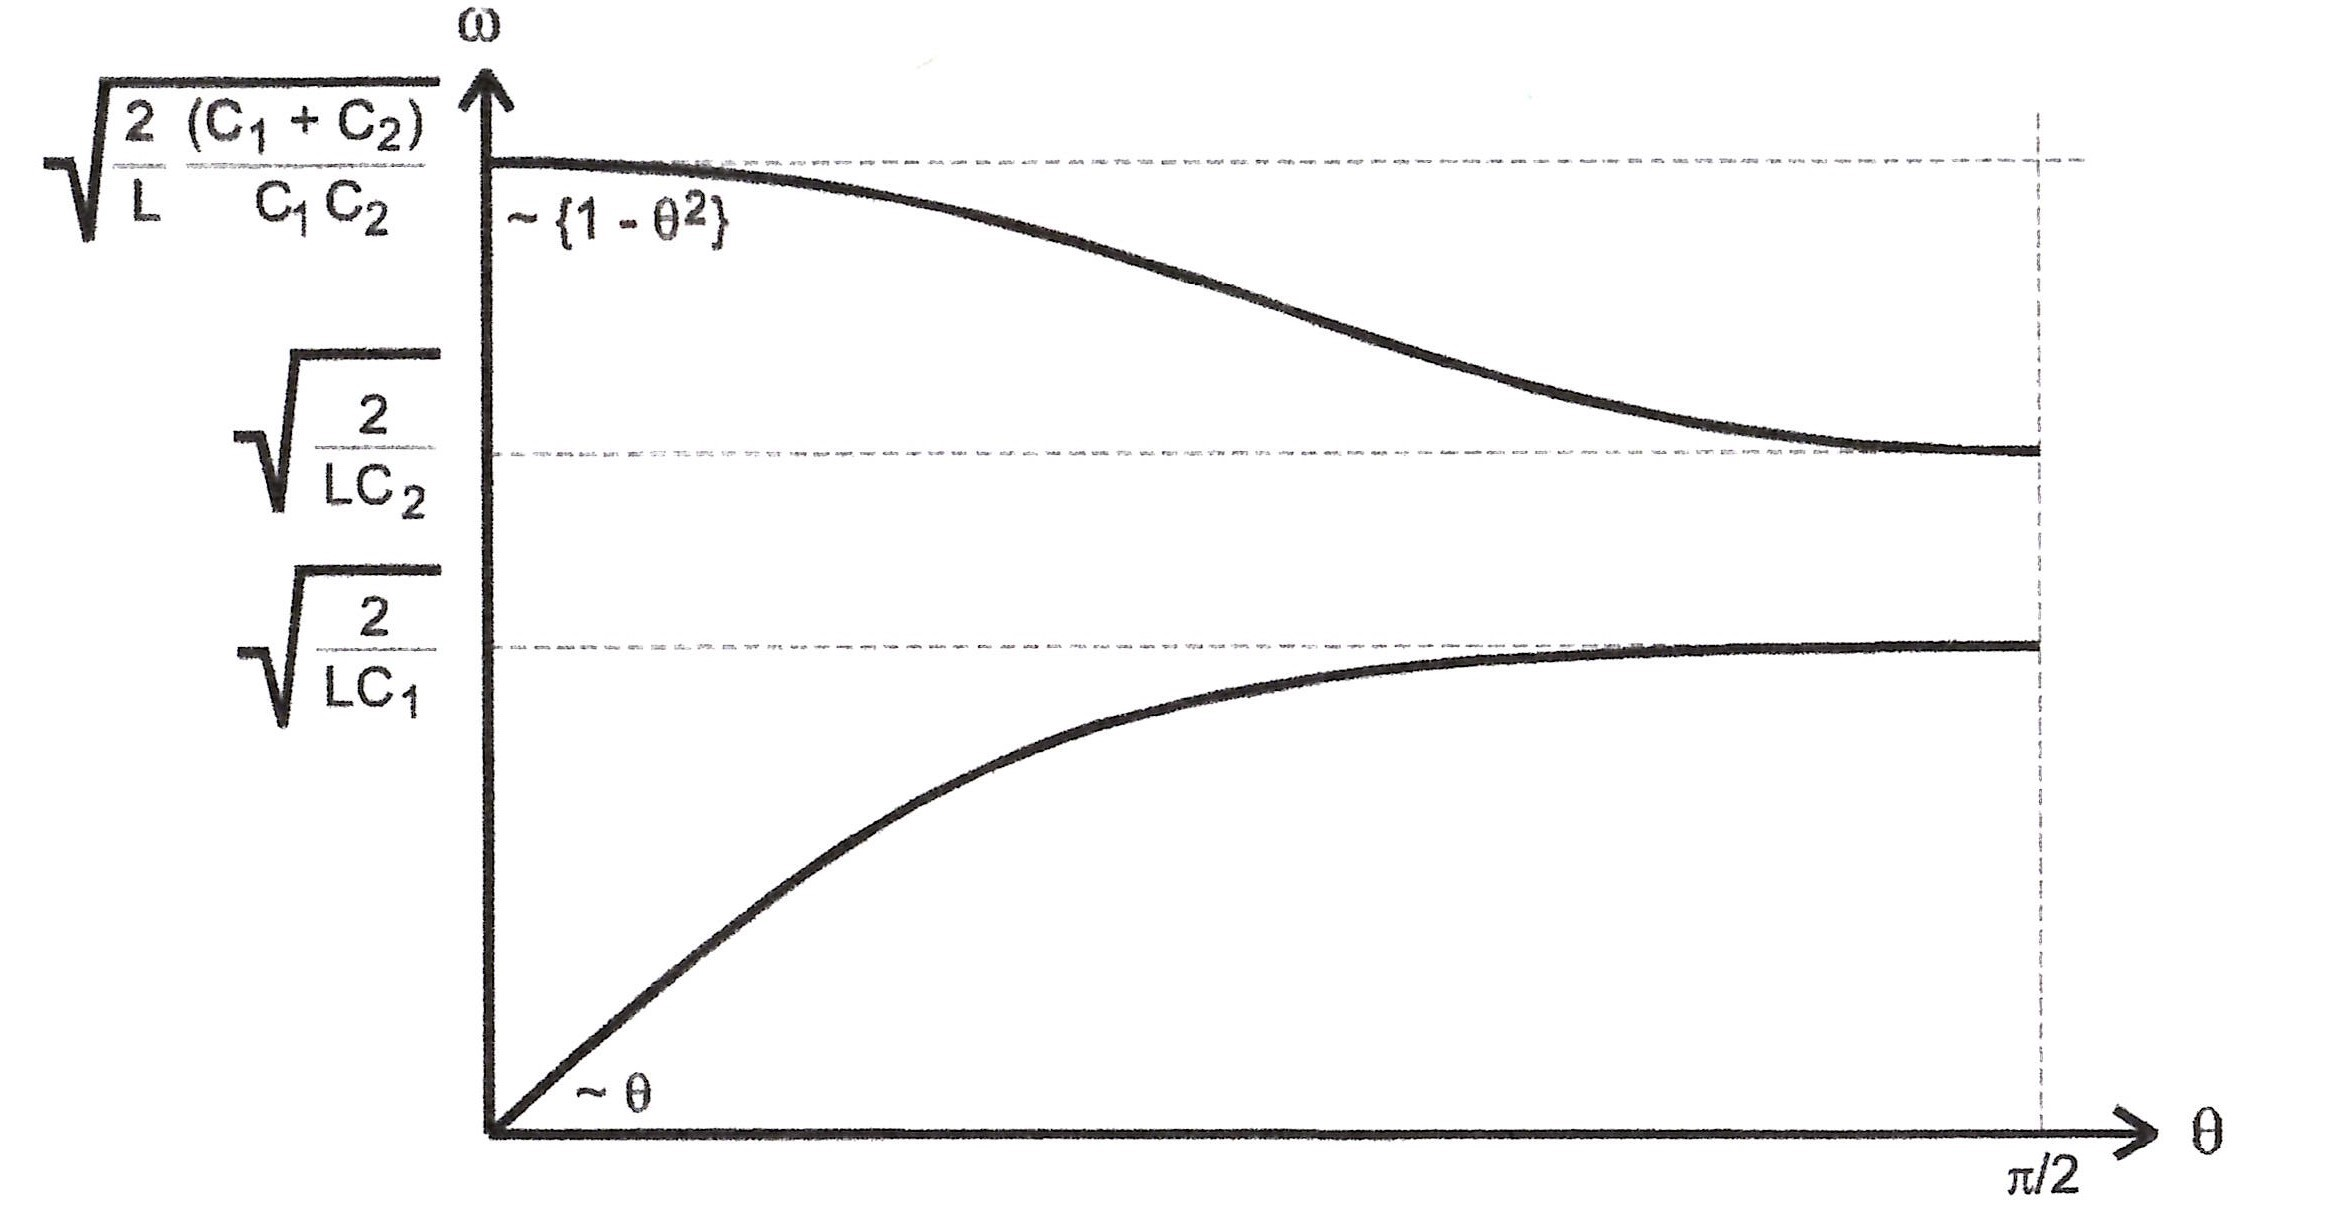
\includegraphics[width = \textwidth]{DIspersionskurveC1C2.jpg}
  \caption{Dispersionskurve bei einer Kette mit zwei unterschiedlichen Kondensatoren \cite{anleitung01}}
  \label{fig:RelationC12}
\end{figure}

Wie der Formel \eqref{eqn:RelationC1C2} entnommen werden kann, bilden sich bei
dieser Dispersionsrelation zwei Äste, auch akustischer und optische Ast genannt
(siehe Abbildung \ref{fig:RelationC12}). Zwischen den beiden Ästen existiert ein Bereich, welcher
bei der Schwingung nicht auftretenden Frequenzen beinhält. Während $\omega\ua{2}$
bei $\theta = \frac{\pi}{2}$ ein Maximum besitzt, tritt dort für $\omega\ua{1}$
ein Minimum auf (siehe Abbildung \ref{fig:RelationC12}).


\begin{align}
  \label{eqn:omega1}
  \omega\ua{1} &= \sqrt{ \frac{1}{L} \frac{2(C\ua{1} + C\ua{2})}{C\ua{1}C\ua{2}}} \,
  \left\{ 1 - \theta^2 \frac{C\ua{1}C\ua{2}}{(C\ua{1} + C\ua{2})^2} \right\} \\
  \label{eqn:omega2}
  \omega\ua{2} &= \sqrt{ \frac{2}{L(C\ua{1} + C\ua{2})}} \, \theta
\end{align}

Aus den Formeln \eqref{eqn:omega1} und \eqref{eqn:omega2} lassen sich nun die in
Abbildung \ref{fig:RelationC12} schon eingetragenen Grenzfrequenzen für den optischen
sowei akustischen Ast bestimmen:

\begin{align}
  \label{eqn:omega_C_grenz}
  \omega_{Grenz,C} &= \frac{2}{\sqrt{L\cdot C_1}} \\
  \label{eqn:omega_C_1_grenz}
  \omega_{Grenz,C_1C_2}^{optisch} &= \sqrt{\frac{2}{L\cdot C_1}}  \\
  \label{eqn:omega_C_2_grenz_unten}
  \omega_{Grenz,C_1C_2,unten}^{akustisch} &= \sqrt{\frac{2}{L\cdot C_2}} \\
  \label{eqn:omega_C_2_grenz_oben}
  \omega_{Grenz,C_1C_2,oben}^{akustisch} &= \sqrt{\frac{2}{L} \frac{(C\ua{1}+C\ua{2})}{C\ua{1}C\ua{2}}}. \\
\end{align}

Aus den bestimmten Dispersionsrelationen lassen sich nun ebenfalls die Phasen- und
die Gruppengeschwindigkeit herleiten. Da die Gruppenheschwindigkeit in dem Versuch
jedoch nicht betrachtet wird, wird im folgenden nur auf die Phasengeschwindigkeit
eingegangen:

\begin{equation}
  v\ua{Ph} = \frac{\omega}{\theta} = \frac{\omega}{\arccos(-\frac{1}{2}\omega^2LC)}
\end{equation}

Die Dispersion verschwindet in dem Bereich kleiner Frequenzen, also bei $\omega$
<< 1/LC. Beim Erreichen der Grenzfrequenz $\omega\ua{G}$ = 2/$\sqrt{\su{LC}}$ erreicht
die Phasengeschwindigkeit einen Minimalwert:

\begin{equation}
  v\ua{Ph\ua{min}} =  \frac{2}{\pi} \frac{1}{\sqrt{\su{LC}}}
  \label{eqn:Phasengeschwindigkeit}
\end{equation}

\subsection{(unendlich lange) LC-Ketten}

Interessant für die Schaltungstechnik ist auch der am Eingang der Kette gemessene
Eingangswiderstand (auch Wellenwiderstand), welcher als Quotient von der am Eingangskondensator anliegenden
Spannung $U\ua{0}$ und dem in die Schaltung hineinfließenden Strom $I\ua{0}$
definiert ist:

\begin{equation}
  Z(\omega) = \frac{U\ua{0}}{I\ua{0}} = \sqrt{ \frac{L}{C}} \frac{1}{ \sqrt{1 - \frac{1}{4} \omega^2 LC} }.
\end{equation}

Der Eingangswiderstand einer (unendlich langen) Kette ist somit rein reell,
obwohl in der Schaltung nur Komponenten mit imaginären Impedanzen verwendet wurden.
Somit sind Strom und Spannung an jedem Ort in
Phase, elektrische Energie kann lediglich in die Kette hineinfließen. Eine
(unendlich lange) Kette kann also auch bei einer begrenzten mit dem Wellenwiderstand
als Abschlusswiderstand simuliert werden.

\begin{figure}
  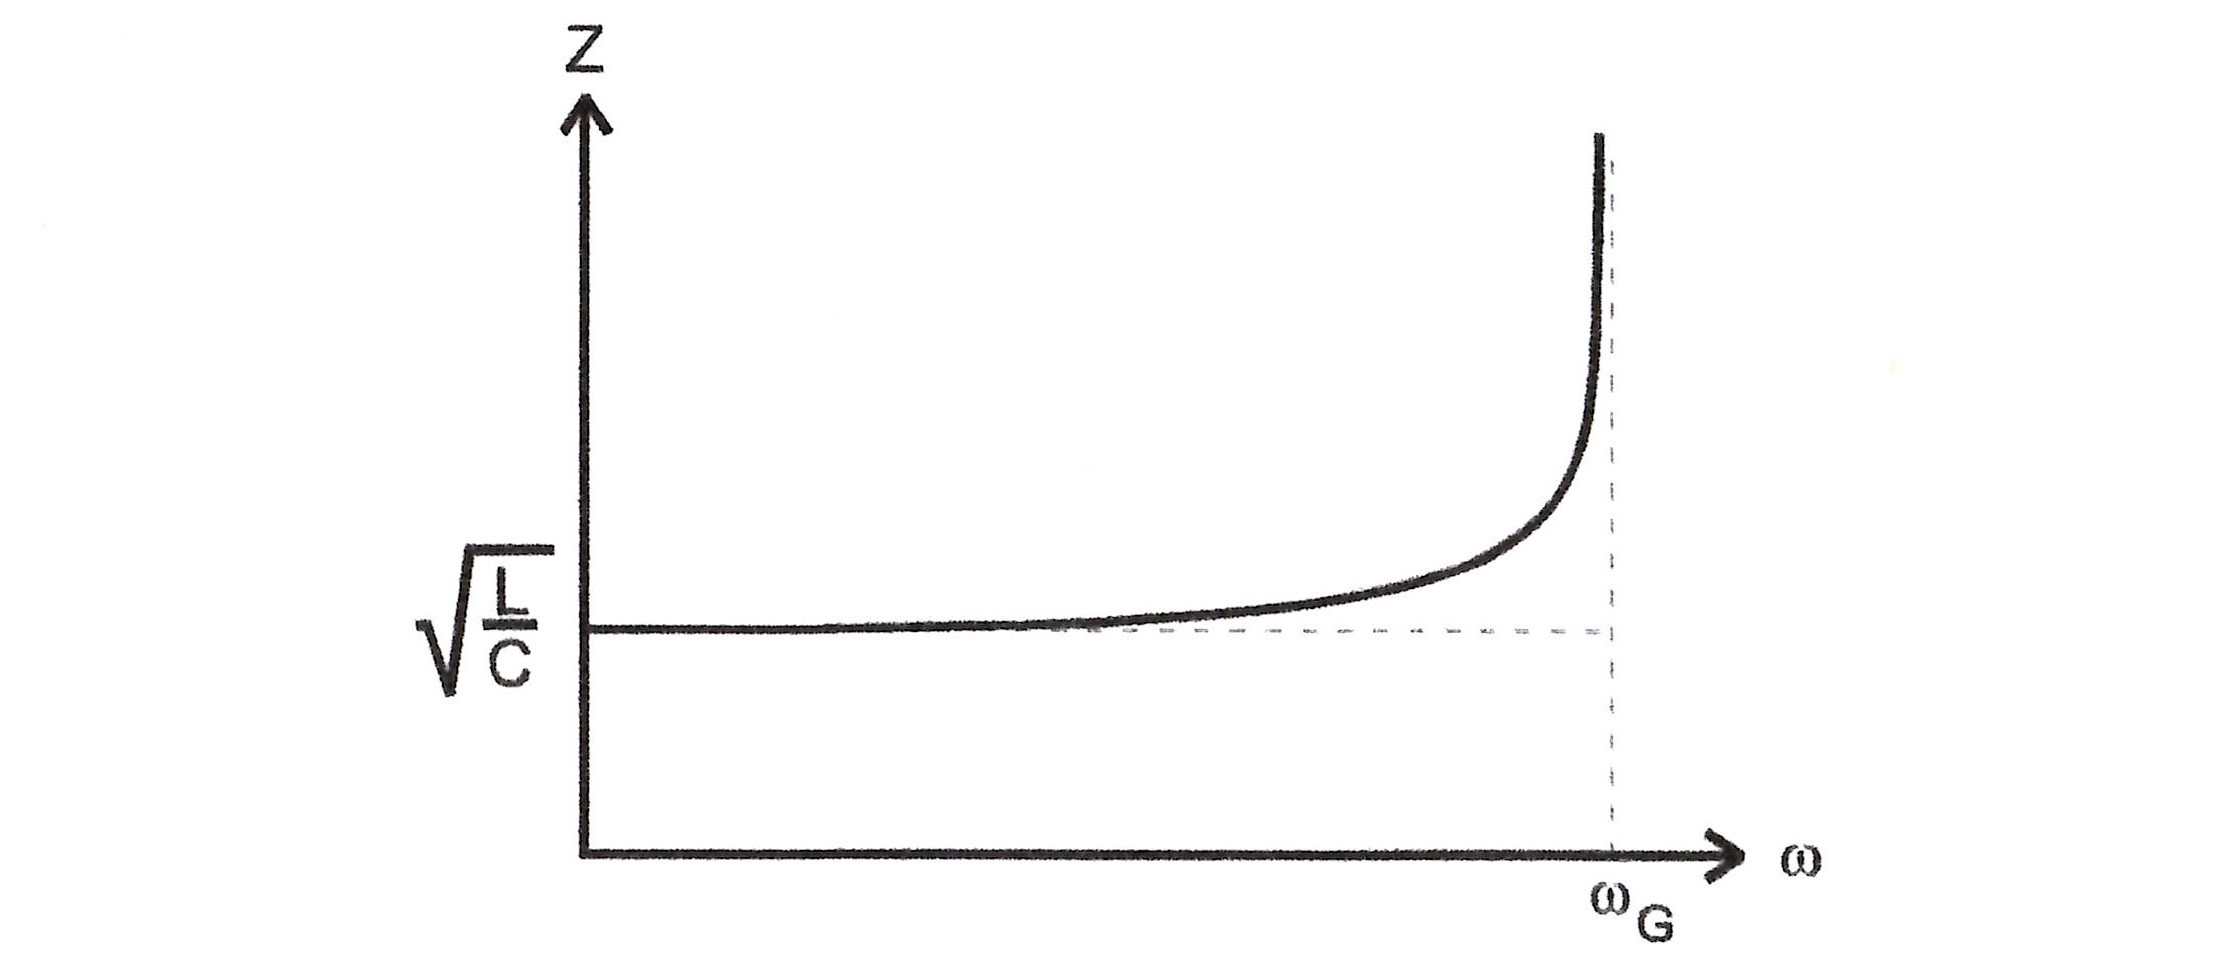
\includegraphics[width = \textwidth]{AbhaengigkeitImpedanz.jpg}
  \caption{Frequenzabhängigkeit der charakteristischen Impedanz \cite{anleitung01}}
  \label{fig:Impedanzabhängigkeit}
\end{figure}

In Abbildung \ref{fig:Impedanzabhängigkeit} sieht man die Abhängigkeit der Impedanz
von der angelegten Frequenz. Zu sehen ist, dass sich die Frequenz einem bestimmten
Grenzwert annähert, ab dem der Wellenwiderstand über alle Grenzen wächst.
Über den angeschlossenen Widerstand und den Wellenwiderstand lässt sich das
Verhältnis zwischen Amplitude der eingehenden und reflektierten Spannung über folgende
Formel bestimmen:

\begin{equation}
  \frac{U\ua{ref}}{U\ua{E}} = \frac{r - Z}{r + Z}.
\end{equation}


Die Welle weist nun für verschiedene Abschlusswiderstände unterschiedliche
Eigenschaften auf, die im folgenden aufgelistet sind:


\renewcommand{\labelenumi}{\alph{enumi})}
\begin{enumerate}
  \item offenes Ende (R = $\infty$): \\
        $U\ua{ref}$ = $U\ua{E}$ $\implies$ vollständige Reflexion ohne Phasensprung.

  \item kurzgeschlossene Kette (R = 0): \\
        $U\ua{ref}$ = - $U\ua{E}$ $\implies$ vollständige Reflexion mit Phasensprung um $\pi$.

  \item Abschluss mit Wellenwiderstand (R = Z): \\
        $U\ua{ref}$ = 0 $\implies$ keine Reflexion.

  \item in allen anderen Fällen tritt eine Teilreflexion auf und bei einem nicht
        reelen R zusätzlich eine Phasendrehung.
\end{enumerate}

Bei den ersten beiden Fällen entsteht durch Interferenz der einlaufenden
und der rücklaufenden Welle eine stehenden Welle.
Dabei entstehen Schwingungsknoten, an denen die Amplitude für alle
Zeiten verschwindet:

\begin{align}
  n\ua{z}\theta &= z \frac{\pi}{2} \, \, \, \, \, (z = 1,3,5, ...)
  \label{eqn:offenesEnde}
\end{align}

\begin{align}
  n\ua{z}\theta &= z \pi \, \, \, \, \, (z = 1,2,3, ...)
  \label{eqn:geschlossenesEnde}
\end{align}

Dabei bezieht sich die Formel \eqref{eqn:offenesEnde} auf ein offenes Ende und
die Formel \eqref{eqn:geschlossenesEnde} auf ein geschlossenes Ende.

Im Fall $R = \infty$ kann sich allerdings nur dann eine stehende Welle ausbilden,
wenn am Kettenende (n=$\su{n}\ua{max}$) ein Spannungsbauch befindet.

\newpage

\section{Versuchsdurchführung}

\subsection{Bestimmung der Durchlasskurve}

\begin{figure}
  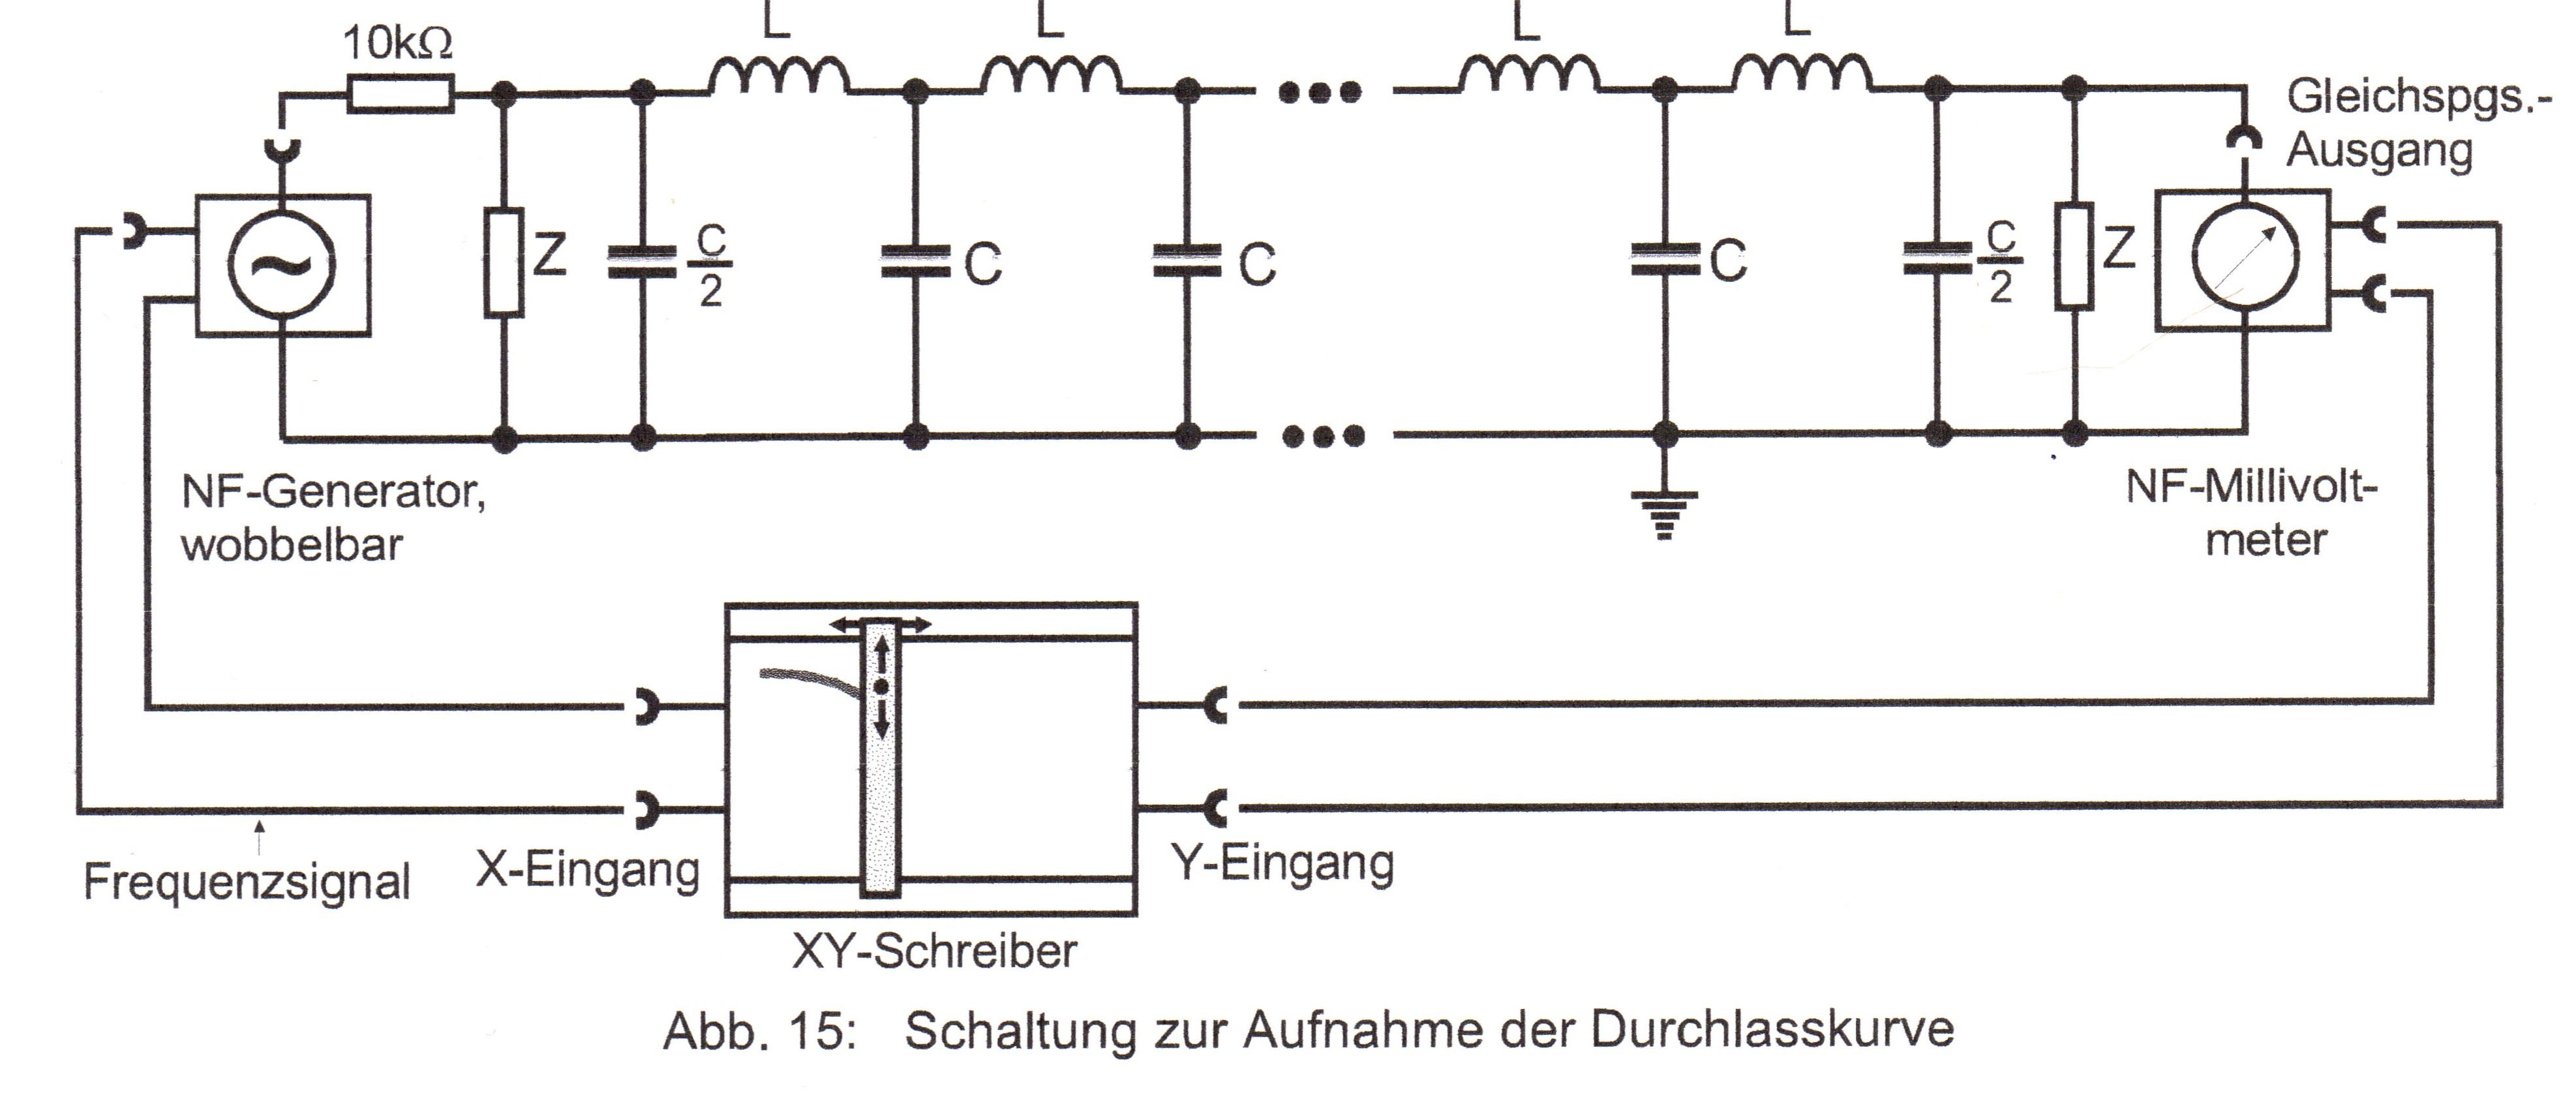
\includegraphics[width = \textwidth]{Durchlasskurve.jpg}
  \caption{Schaltung zur Bestimmung der Durchlasskurve und dem Nachweis stehender Wellen \cite{anleitung01}}
  \label{fig:Durchlasskurve}
\end{figure}

In dem ersten Teil des Experimentes wird mithilfe eines Schreibers eine Durchlasskurve
für beide Ketten angefertigt. Dabei wird an dem Generator ein Sweep eingestellt,
sodass der Schreiber die gemessenen Spannungamplitude am Ausgang der LC-Kette in Abhängigkeit
der anliegenden Frequenz aufzeichnet. Dabei müssen die Achsen so angepasst sein,
dass die Grenzfrequenzen auf der angefertigten Zeichnung ebenfalls zu sehen sind.
Die Schaltung für diesen Teil der Messung ist in Abbildung \ref{fig:Durchlasskurve}
zu sehen.


\subsection{Bestimmung der Dispersionsrelation}

\begin{figure}
  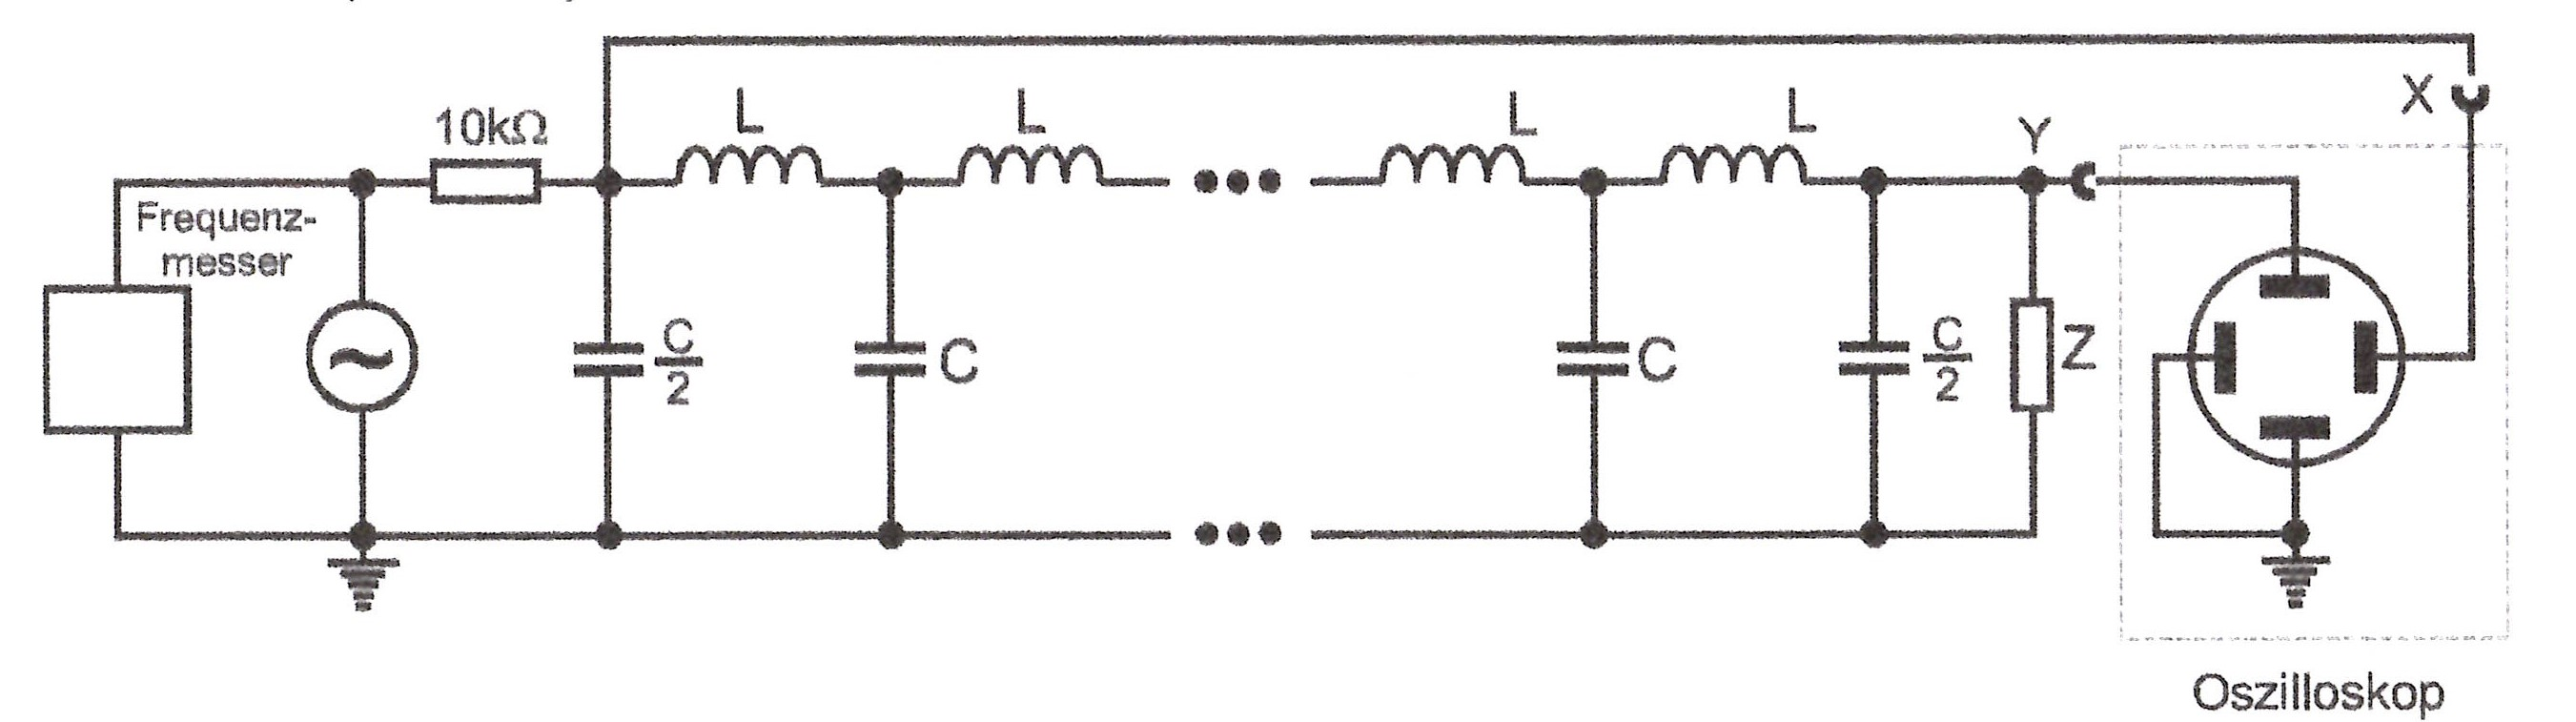
\includegraphics[width = \textwidth]{Dispersionsrelation.jpg}
  \caption{Schaltung zur Bestimmung der Dispersionsrelation \cite{anleitung01}}
  \label{fig:Dispersion}
\end{figure}

Mithilfe der in Abbildung \ref{fig:Dispersion} dargestellten Schaltung lässt sich
die Phasenverschiebung
pro Kettenglied betrachten. Dafür wird an einem Oszillloskop mithilfe von Lissajous-Figuren
die Phasenverschiebung zwischen Eingangs- und Ausgangsspannung betrachtet, wobei
lediglich Frequenzen mit einer Phasenverschiebung eines Vielfachen von $\pi$
notiert werden.


\subsection{Nachweis von stehenden Wellen}

Mit der Schaltung nach Abbildung \ref{fig:Durchlasskurve} (ohne Schreiber und Wobbeleinrichtung) wird
nun versucht, stehende Wellen nachzuweisen.
Dafür wird mit einem Millivoltmeter anfangs die Ausgangsspannung gemessen, um eine
Frequenz mit einem Spannungsmaximum am Kettenende zu finden. Danach wird an jedem
Kettenglied die auftretende Spannung gemessen. Diese Messung wird für eine
beiderseits offene Kette mit der 1. und 2. Eigenschwingung durchgeführt und danach
für eine mit dem Wellenwiderstand als Abschlusswiderstand eingestellte Kette
für eine beliebige Eigenfrequenz wiederholt.

\newpage

\section{Auswertung}

Die verwendeten Zylinder wurden mithilfe einer Schieblehre vermessen und
hatten die folgenden Längen. Dabei werden die Werte als fehlerfrei angenommen.

\begin{description}
  \item[Zylinder 1] \SI{40,35}{\milli\meter}
  \item[Zylinder 2] \SI{80,55}{\milli\meter}
  \item[Zylinder 3] \SI{80,45}{\milli\meter}
  \item[Zylinder 4] \SI{102,1}{\milli\meter}
  \item[Zylinder 5] \SI{31,1}{\milli\meter}
  \item[Zylinder 6] \SI{39,7}{\milli\meter}
  \item[Zylinder 7] \SI{61,5}{\milli\meter}
\end{description}

\subsection{Bestimmung der Dämpfungskonstante und der Schallgeschwindigkeit mit dem Impuls--Echo--Verfahren}

Die Dämpfungskonstante $\alpha$ aus \eqref{eqn:Intensität}
lässt sich aus den genommenen Daten berechnen. Dafür werden die Messdaten
in die Formel \eqref{eqn:Intensität} eingesetzt und wie folgt nach $\alpha$ aufgelöst.

\begin{equation}
  \label{eqn:dämpfung}
  \alpha = - \frac{1}{x_1} \ln{\left(\frac{I_0^\text{'}}{I_0}\right)}
\end{equation}

Dabei ist $I_0^\text{'}$ die Amplitude an der Stelle $x_1 > 0$ und $I_0$
die Amplitude an der Stelle $x  = 0$.

Die Messdaten sind in Tabelle \ref{tab:Messdaten} dargestellt.
Die Werte für Zylinder 4 und den zusammengesetzten Zylinder mit dem
achten Messwert wurden für die Berechnung der Dämpfungskonstante nicht
verwendet, weil die Peaks nur bei Verstärkug ausgemessen werden konnten.
Auf das Herausrechnen des Verstärkungsfaktors wurde der Einfachheit halber verzichtet.
Im Mittel ergibt sich die Dämpfungskontante zu:

\begin{equation}
  \alpha = \SI{21.257(301)}{\per\meter}.
\end{equation}

Der Fehler ist die Standardabweichung des Mittelwertes.
Eine Darstellung der Dämpfung in Acryl ist in dem Diagramm \ref{fig:Dämpfung}
einzusehen. Dabei sind die Messdaten der Anfangs- und Endamplituden
ebenfalls eingetragen.


\begin{figure}
  \centering
  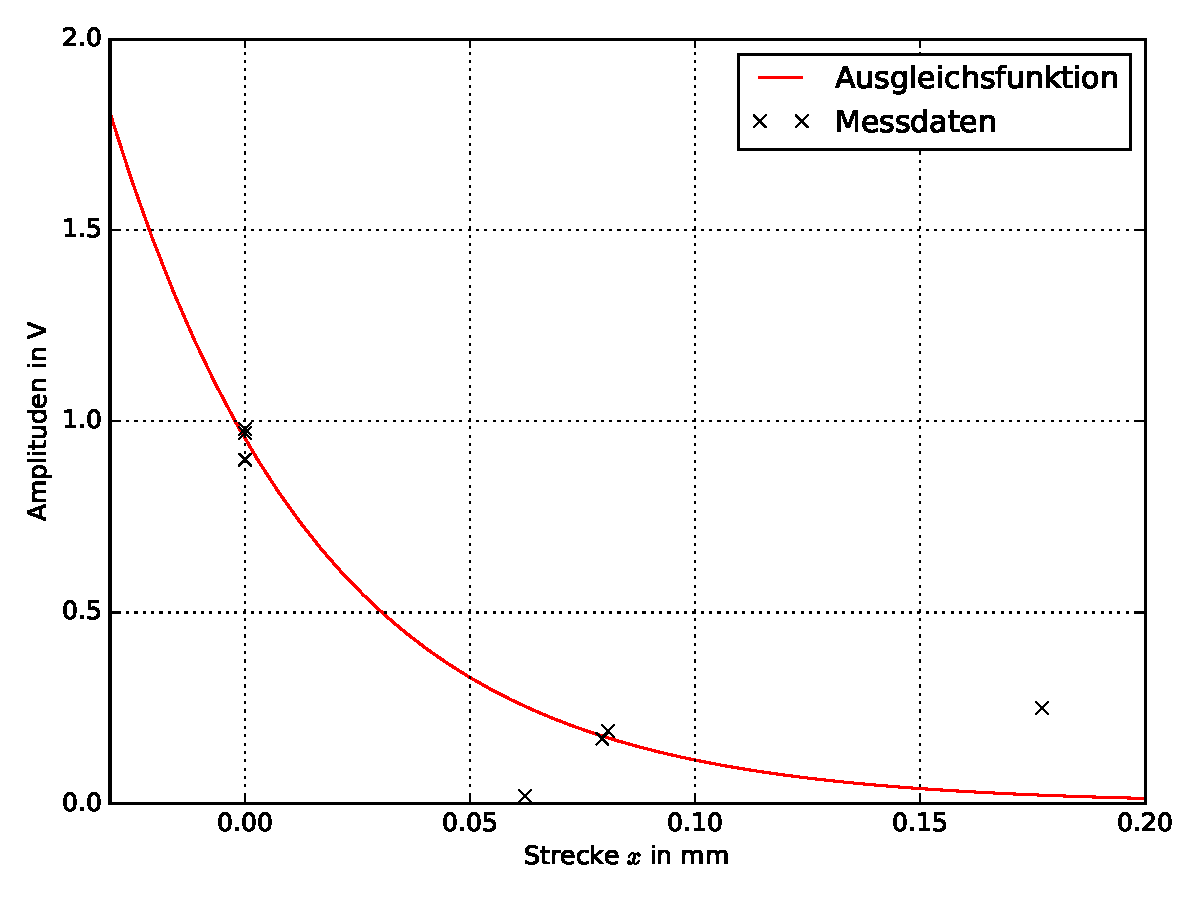
\includegraphics[width=\textwidth]{Pics/Daempfung.pdf}
  \caption{Darstellung der Dämpfung der Amplitude mit Zunahme der Strecke.}
  \label{fig:Dämpfung}
\end{figure}

Die Schallgeschwindigkeit ist aus den Laufzeiten zwischen den
gemessenen Peaks und den vermessenen Zylinderlängen mithilfe von
\eqref{eqn:Fehlstelle} zu berechnen. Dafür wurde mit dem
\emph{Python}-Packet \emph{curve\_fit} eine lineare Ausgleichsrechnung
durchgeführt. Der systematische Fehler der Sonde ist der Ordinaten-Abschnitt
der Ausgleichgeraden und die Schallgeschwindigkeit ist in der Steigung
wiederzufinden.

Die Werte ergeben sich zu:

\begin{align}
  \label{eqn:schallgesch_echo}
  c\ua{Acryl, echo} &= \SI{2880.943}{\meter\per\second} \\
  \Delta\ua{Sonde,echo} &= \SI{-3.862}{\meter\per\second}.
\end{align}

Das zugehörige Diagramm der Messung ist im Folgenden dargestellt.

\begin{figure}
  \centering
  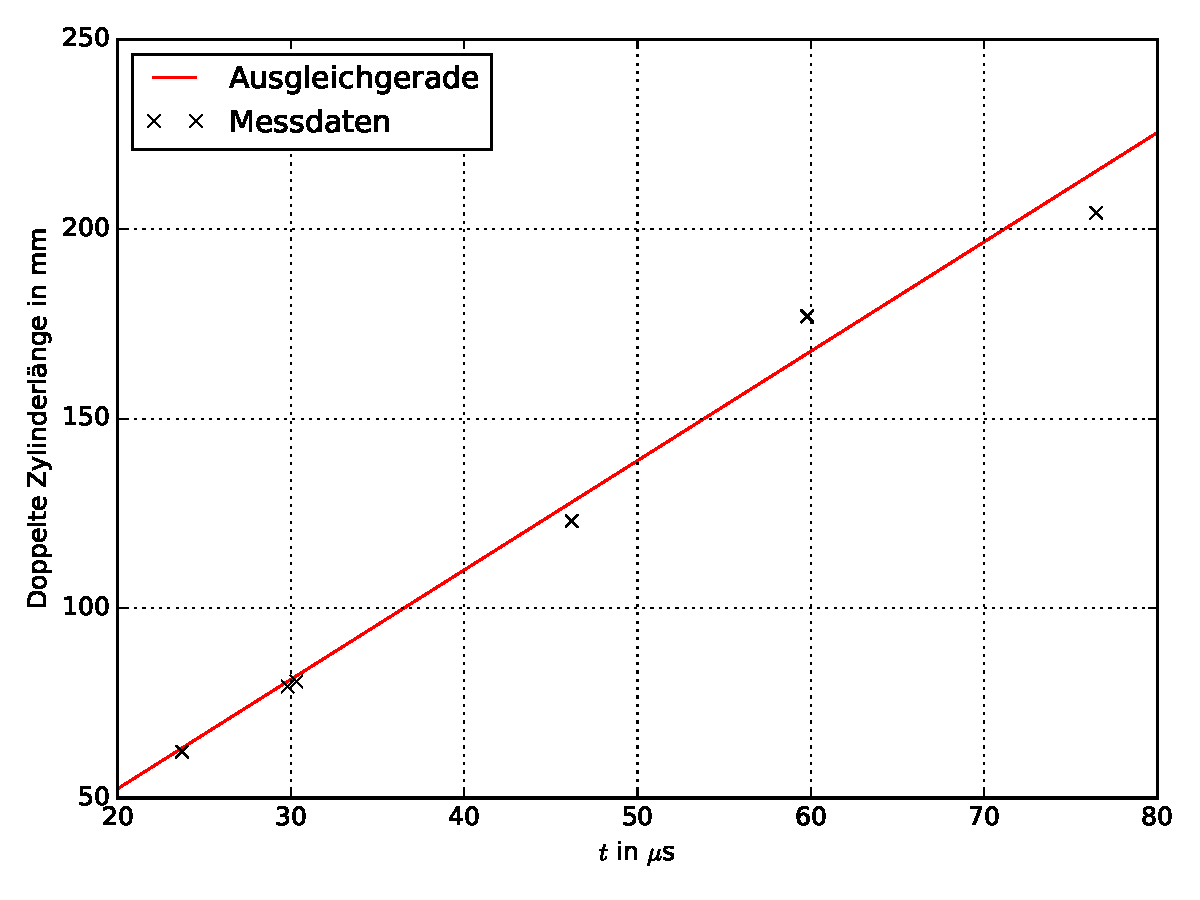
\includegraphics[width=\textwidth]{Pics/schallgesch_echo.pdf}
  \caption{Schallgeschwindigkeit in Acryl, bestimmt über das Impuls-Echo-Verfahren.}
  \label{fig:schallgesch_echo}
\end{figure}

\begin{table}
\centering
\caption{Messdaten zu dem Impuls-Echo-Verfahren. Die Werte sind den Zylindern 1 - 7 derReihe nach zuzuordnen. Der achte Messert entspricht einem Zylinder der Länge $\su{Z}_1 + \su{Z}_7$.}
\label{tab:Messdaten}
\begin{tabular}{S S S S}
\toprule
{$\su{U}\ua{1}$ in $\si{\volt}$} & {$t_1$ in $\si{\mu\second}$} & {$\su{U}\ua{2}$ in $\si{\volt}$} & {$t_2$ in $\si{\mu\second}$}  \\
\midrule
 0.90  & 0.40  & 0.17  & 30.30\\
0.97  & 0.40  & 0.02  & 59.80\\
0.98  & 0.50  & 0.01  & 59.80\\
1.00  & 0.40  & 0.12  & 76.49\\
0.97  & 0.40  & 0.25  & 23.70\\
0.98  & 0.50  & 0.19  & 29.80\\
0.97  & 0.40  & 0.04  & 46.20\\
1.00  & 0.50  & 0.12  & 75.70\\
\bottomrule
\end{tabular}
\end{table}

\FloatBarrier

\subsection{Bestimmung der Schallgeschwindigkeit mit dem Durchschallungsverfahren}

Die Messdaten zum Durchschallungsverfahren sind in Tabelle \ref{tab:durchschall}
dargestellt.
Es wurde gleich verfahren wie bei dem Impuls-Echo-Verfahren.

Die Werte ergeben sich zu:

\begin{align}
  \label{eqn:schallgesch_durch}
  c\ua{Acryl, durch} &= \SI{2878.377}{\meter\per\second} \\
  \Delta\ua{Sonde, durch} &= \SI{-2.946}{\meter\per\second}.
\end{align}

Das zugehörige Diagramm der Messung ist im Folgenden dargestellt.

\begin{figure}
  \centering
  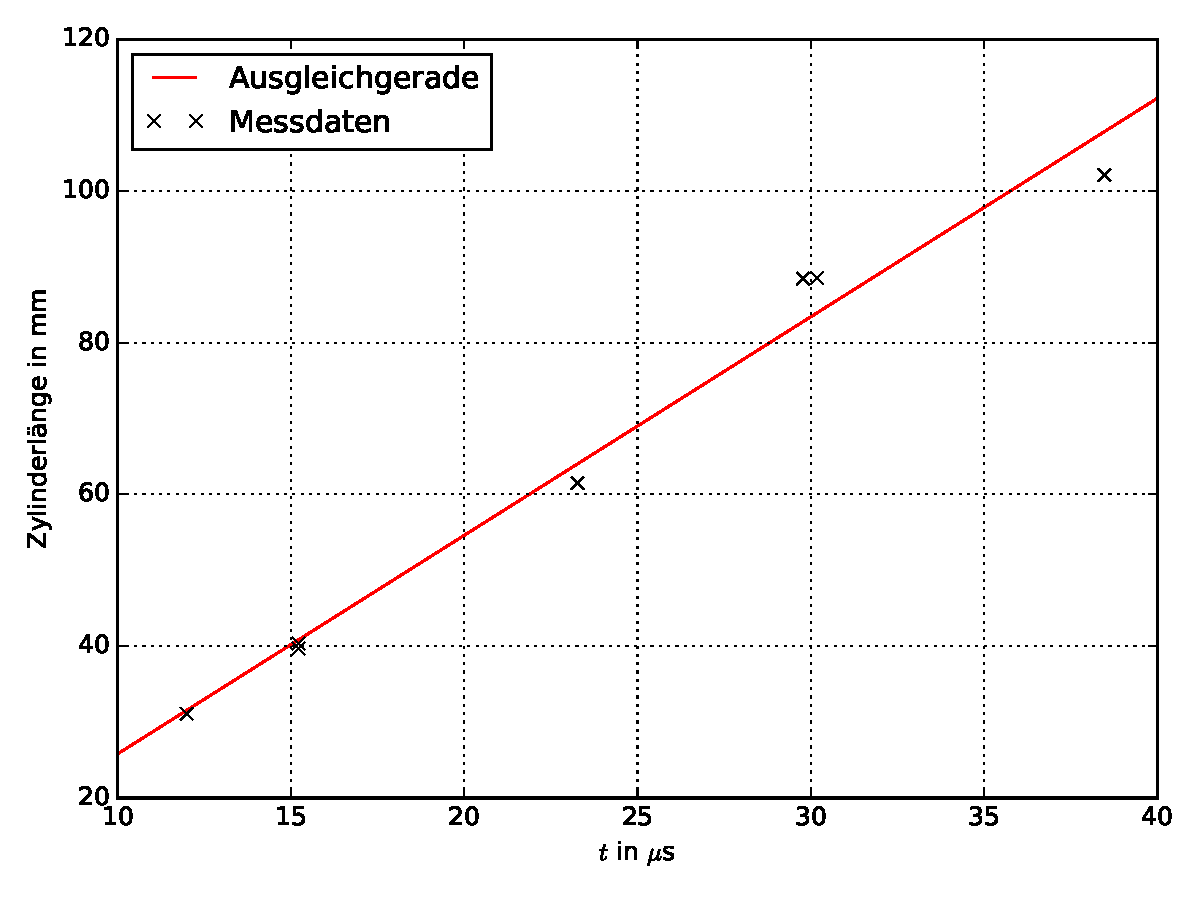
\includegraphics[width=\textwidth]{Pics/schallgesch_durch.pdf}
  \caption{Schallgeschwindigkeit in Acryl, bestimmt über das Durchschallungsverfahren.}
  \label{fig:schallgesch_durch}
\end{figure}

\begin{table}
\centering
\caption{Messdaten zu dem Durchschallungsverfahren. Die Messdaten sind der Reihe nach den Zylindern 1 - 7 zuzuordnen.}
\label{tab:durchschall}
\begin{tabular}{S }
\toprule
{Laufzeiten in \si{\mu\second}}  \\
\midrule
 15.21\\
29.78\\
30.18\\
38.48\\
11.98\\
15.21\\
23.27\\
\bottomrule
\end{tabular}
\end{table}

\FloatBarrier

\subsection{Spektrale Analyse und Cepstrum}

Die verwendeten Acrylplatten wurde mit einer Schieblehre vermessen.
Die Dicken wurden ebenfalls als fehlerfrei angenommen.

\begin{description}
  \item[Platte 1] $d_1 = \SI{9.9}{\milli\meter}$
  \item[Platte 2] $d_2 = \SI{6}{\milli\meter}$
\end{description}

Das Durchschallungsverfahren ergab die folgenden Werte.

\begin{description}
  \item[Platte 1] $d_1 = \SI{10.51}{\milli\meter}$
  \item[Platte 2] $d_2 = \SI{6.48}{\milli\meter}$
\end{description}

Die bestimmten Werte weichen um $\Delta\ua{Platte 1} = \SI{0.61}{\milli\meter}$
und $\Delta\ua{Platte 2} = \SI{0.48}{\milli\meter}$ von den mit der
Schieblehre vermessenen Werten ab.

Die Fehler aus dem systematische Fehler der Sonde sind vernachlässigbar klein.

Das Spektrum und das Cepstrum wurden aufgenommen. Die genommenen
Diagramme sind im Folgendem dargestellt.

\begin
{figure}
\centering
\begin{subfigure}{0.48\textwidth}
\centering
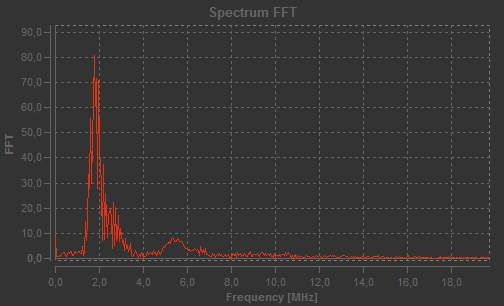
\includegraphics[height=4.2cm]{Pics/Z6_M3_S.jpg}
\caption{Aufgenommenes Spektrum.}
\label{fig:Spektrum}
\end{subfigure}
\begin
{subfigure}{0.48\textwidth}
\centering
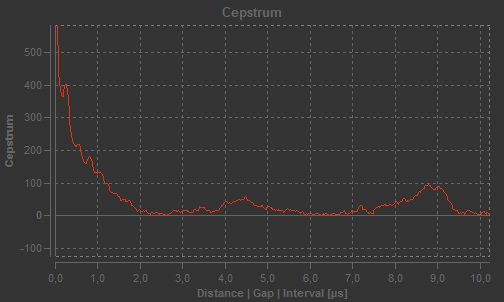
\includegraphics
[height=4.2cm]{Pics/Z6_M3_C.jpg}
\caption{Aufgenommenes Cepstrum.}
\label{fig:Cepstrum}
\end{subfigure}
\end{figure}

\subsection{Biometrische Untersuchung eines Augenmodells}

Es wurde ein Auge wie aus Abb. \ref{fig:Auge} untersucht.
Insgesamt wurden fünf Peaks aufgenommen die den folgenden Bestandteilen des Auges
zuzuordnen sind.

\begin{enumerate}
  \item Hornhaut
  \item Iris
  \item Linseneingang
  \item Linsenausgang
  \item Retina
\end{enumerate}

Die Peaks spiegeln der Aufzählung entsprechend die Bestandteilen des Auges wieder.
Für die Bereiche zwischen Hornhaut und Linseneingang, sowie
Linsenausgang und Retina wurde die Schallgeschwindigkeit für
Glaskörper verwendet ($c\ua{Glaskoerper} = \SI{1410}{\meter\per\second}$
\cite{anleitung01}).
Für den Bereich zwischen Linseneingang und Linsenausgang
wurde eine Schallgeschwindigkeit von $c\ua{Linse} = \SI{2500}{\meter\per\second}$
angenommen.

Die Bestandteile des Auges haben die folgenden Tiefen.

\begin{description}
  \item[Hornhaut] $\SI{0}{\milli\meter}$
  \item[Iris] $\SI{4.385(11)}{\milli\meter}$
  \item[Linseneingang] $\SI{7.635(18)}{\milli\meter}$
  \item[Linsenausgang] $\SI{14.835(21)}{\milli\meter}$
  \item[Retina] $\SI{44.23(9)}{\milli\meter}$
\end{description}

Die dazugehörigen Fehler entstehen durch den systematischen Fehler der Sonde.

Die Messdaten sind in der Tabelle \ref{tab:Auge} einzusehen.

\begin{table}
\centering
\caption{Messdaten zur biometrischen Untersuchung des Auges. Die Messdaten sind der Reihe den Bestandteile des Auges zuzuordnen.}
\label{tab:Auge} 
\begin{tabular}{S S }
\toprule
{Peakabstand $\Delta_{\symup{peak}}$ in \si{\mu\second}}  & {Absoluter Abstand}  \\
\midrule
 0.20  & 0.20\\
6.22  & 6.64\\
4.61  & 11.05\\
5.76  & 16.81\\
41.70  & 70.26\\
\bottomrule
\end{tabular}
\end{table}


\section{Diskussion}

Als Literaturwert der Schallgeschwindigkeit in Acryl wurde
$c\ua{Acyl, lit} = \SI{2730}{\meter\per\second}$\cite{lit} angenommen.
Die Schallgeschwindigkeit in Acryl wurde über zwei verschiedenen
Ultraschallverfahren ermittelt. Die berechneten Werte unterscheiden sich
um $\Delta\ua{c, gemessen} = \SI{1.740(917)}{\meter\per\second}$.
Hingegen liegt der Unterschied des gemittelten Wertes zum Literaturwert bei $\SI{149.246(3404)}{\meter\per\second}$.
Da beide Verfahren einen deutlichen Unterschied zu dem Literaturwert aufweisen,
aber untereinander kaum verschieden sind, wird
ein weiterer systematischer Fehler, der von dem systematischen Fehler der
Sonde verschieden ist angenommen.
Die Dicke der Acrylplatten wurden einmal über eine Schieblehre und
zum anderen über das Durchschallungsverfahren ermittelt.
Die Dicken, die sich aus dem Durchschallungsverfahren ergeben, sind
ca. einen halben Millimeter größer als die ausgemessenen Werte.
Mit dem Literaturwert für die Schallgeschwindigkeit von Acryl
ergeben sich die Plattendicken zu:

\begin{description}
  \item[Platte 1] $d_1 = \SI{9.96}{\milli\meter}$
  \item[Platte 2] $d_2 = \SI{6.14}{\milli\meter}$.
\end{description}

Damit ist die Abweichung der Plattendicken auf den systematischen Fehler
der Schallgeschwindigkeit zurückzuführen.

Die Diagramme aus der Spektralen Analyse (\ref{fig:Spektrum}, \ref{fig:Cepstrum})
werden im Folgenden diskutiert. In dem Diagramm des Cepstrums sind nicht die Lagen der tatsächlich
beobachteten Peaks erkenntlich, hingegen werden Peaks dargestellt, die
nicht beobachtet wurden. Das Spektrum zeigt einen Peak bei ca. $\SI{1.8}{\mega\hertz}$.
Die Eingangsfrequenz betrug hingegen $\SI{2}{\mega\hertz}$. Die weiteren Peaks
sind durch Reflexionen der Eingangswelle zu erklären.

Die biometrische Untersuchung des Auges ergab Werte, die
mit den Erwartungswerten übereinstimmen. Hierbei muss der
systematische Fehler ebenfalls bedacht werden, weshalb davon auszugehen
ist, dass die tatsächlichen Werte kleiner als die bestimmten Werte sind.


\printbibliography

\end{document}
